\chapter{توضیح مختصری بر الگوریتم}

در فصل \ref{ch:rl} در مورد مفاهیم \w{rl} بحث شد. مهمترین مفاهیم عبارتند از:
\begin{multicols}{3}
\begin{enumerate}
	\item \w{env} \item \w{agent} \item \w{env state} \item \w{agent state} \item \w{reward} \item \w{observ} 
\end{enumerate}
\end{multicols}

هدف در این پروژه این بود که یک \w{autocar} با استفاده از الگوریتم های \w{rl} ساخته شود. جزییات تئوری الگوریتم و جزییات فنی پروژه به ترتیب در بخش های 
\ref{ch:rl}
و
\ref{ch:fani}
آورده شده‌اند.
در این بخش به شبیه سازی و جزییات کار و تعریف پارامتر های این پروژه برداخته می‌شود.

\section{معرفی محیط شبیه سازی}

در ابتدا محیط شبیه سازی را معرفی می‌کنیم. جزییات فنی این محیط در \ref{ch:fani} و همچنین نحوه راه‌اندازی آن در بخش \ref{ch:resault|sec:launch} به‌صورت کامل مورد بحث قرار گرفته است. اگر آن محیط را باز کنید محیط مانند شکل 
\ref{fig:obs-1}
باز خواهد شد. این محیط دو آبجکت مهم دارد؛
\begin{alphinline}
	\item ماشین(اتومبیل)
	\item جاده
\end{alphinline}
(شکل \ref{fig:road-car-models}) 



\begin{figure}
	\centering
	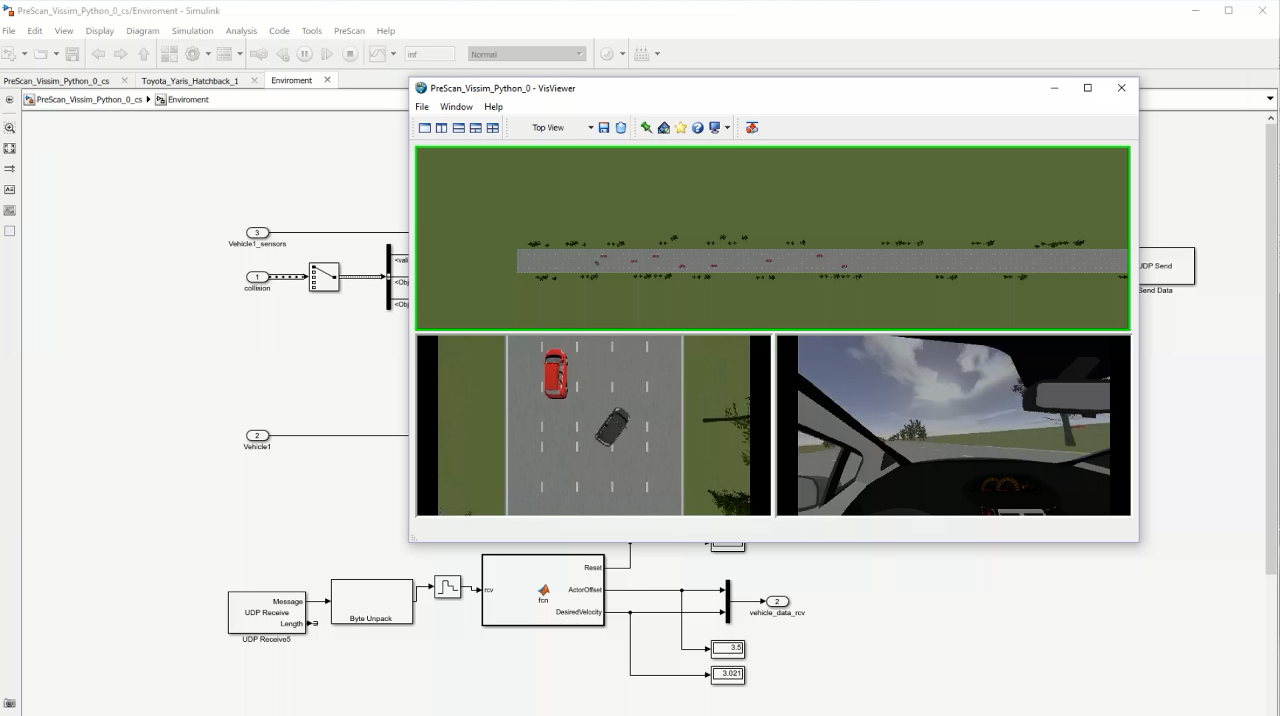
\includegraphics[width=0.7\linewidth]{Figures/OBS/1}
	\caption{محیط شبیه سازی}
	\label{fig:obs-1}
\end{figure}


%HERE
\begin{figure}
	\centering
	\def\localheight{2cm}
	\subfigure[]{%
		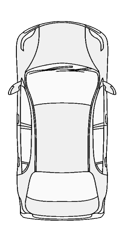
\includegraphics[height=\localheight]{Figures/rzbinary/agent}
		\label{subfig:model-car}
	}
	\hspace*{0.5cm} % space between two figures
	\subfigure[]{%
		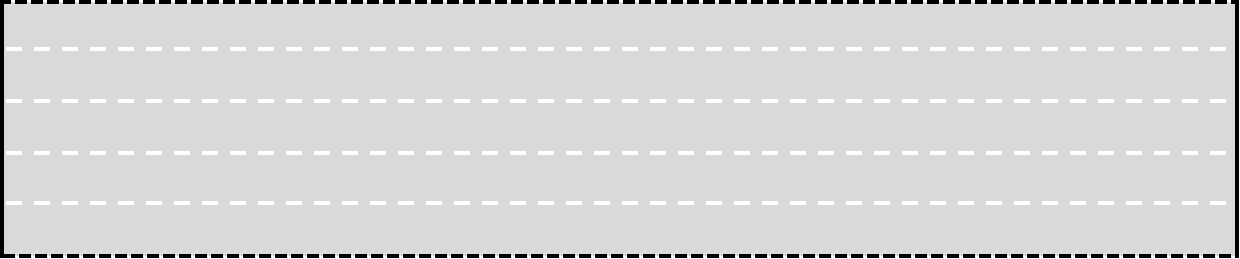
\includegraphics[height=\localheight]{Figures/rzbinary/road}
		\label{subfig:model-road}
	}
	\caption[]{%
	}
	\label{fig:road-car-models}
\end{figure}


چیزی که اهمیت دارد اندازه ها و نحوه تعریف محدوده هاست. شکل \ref{fig:road-car-total} اندازه‌ها و محدوده ها را مشخص کرده است. 
شکل \ref{subfig:road-car-redbox-w} نشان می‌دهد که این محدوده ها کاملا برروی یک دیگر منطبق نیستند. دلیل اصلی این موضوع عدم اهمیت تطبیق دقیق این دو می‌باشد. در بخشی که پشت ماشین قرار دارد این محدوده از $-4$ (کمی بیشتر از اندازه عرض لاین ها) شروع می‌شود. زیرا نیازی نیست بیشتر از این مقدار ماشین مورد بررسی به عقب برود تا متوجه شویم اشتباه در حال رفتن است. درحقیقت این مورد کمک می‌کند تا تعداد \w{step} ها را در هر \w{episode} اشتباه کاهش یابد. بخش های کناری نیز از $-11$ تا $+11$ محدود شده‌اند (بیشتر از عرض خود جاده) تا اگر نوسانی یافت به ماشین این اجازه داده شود تا به مسیر اصلب برگردد. 







\begin{figure}
	\centering
%	\def\localdata{}
	\subfigure[]{%
		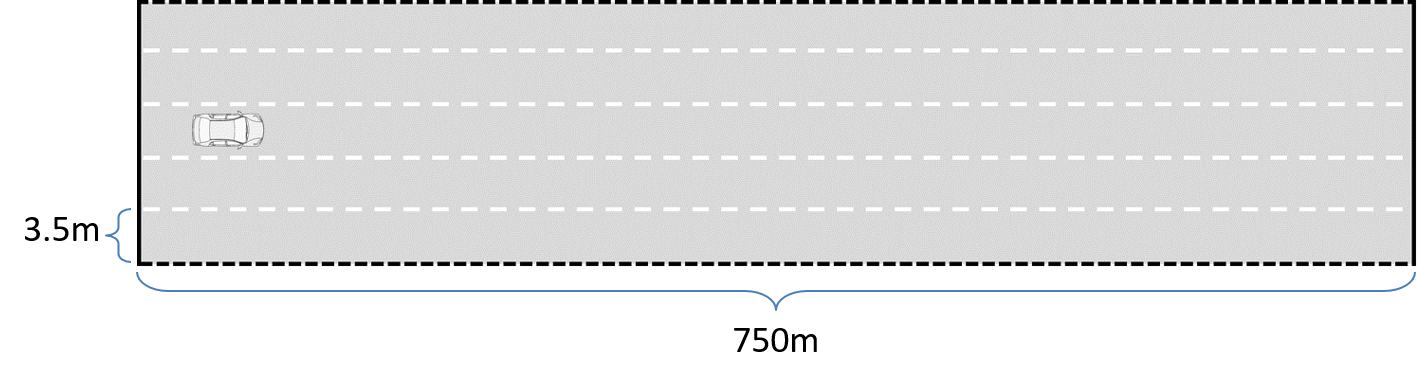
\includegraphics[width=0.7\linewidth]{Figures/rzbinary/road-car-wh}
		\label{subfig:road-car-wh}
	}
	%  	\hspace*{1.5cm} % space between two figures
	\subfigure[]{%
		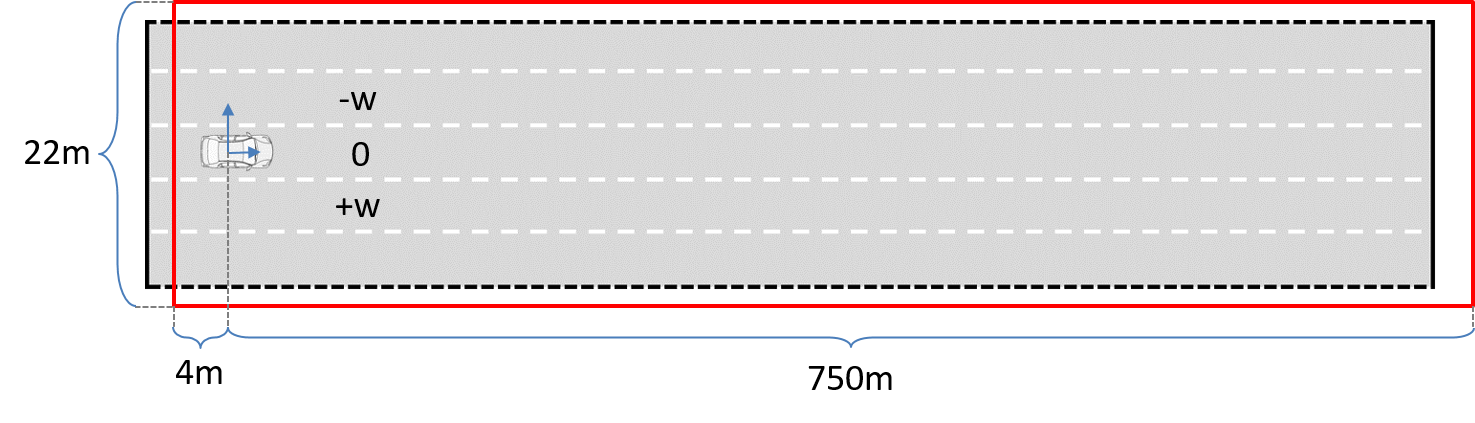
\includegraphics[width=0.7\linewidth]{Figures/rzbinary/road-car-redbox+-w}
		\label{subfig:road-car-redbox-w}
	}
	\caption[]{%
	}
	\label{fig:road-car-total}
\end{figure}

3 مقدار \lr{+w} ، \lr{-w} و \lr{0} که در شکل \ref{subfig:road-car-redbox-w} بر روی جاده نوشته شده است در حقیقت مرتبط با بحث فنی ماجرا می‌باشد اما مفهوم آن این است که \w{agent} مورد بررسی می‌تواند این سه لاین را به عنوان \w{action} اختیار کند. در این مورد بیشتر صحبت خواهد شد.


\code{dqn-train.py}





\section{تعریف کردن پارامتر های \ws{rl}}
ابتدا پارامترهای \w{rl} را مورد بررسی قرار می‌دهیم.
\footnote{منظور از پارامتر های \w{rl} پارامتر هایی مانند تعیین \w{reward} و \w{state} می‌باشد.
}
